\documentclass[12pt,a4paper,twopage]{article}
\usepackage[utf8]{inputenc}
\usepackage{geometry}
\geometry{a4paper,left=30mm,right=30mm, top=3cm, bottom=30mm} 
\usepackage{multicol}
\usepackage{amsmath}
\usepackage{float}
\usepackage{epsfig,graphicx}
\usepackage{xcolor,import}
\usepackage{subcaption}
\usepackage[font=small,labelfont=bf]{caption}
\usepackage{siunitx}
\usepackage[german]{babel}
\usepackage{textcomp}
\usepackage{mathtools}
\linespread{1.1}
\usepackage{parskip}
%\setlength{\parskip}{14pt}
\setlength{\parindent}{12pt}

\begin{document}

\begin{verbatim}


\end{verbatim}

\thispagestyle{empty}
			\begin{center}
			\Large{Fakultät für Physik}\\
			\end{center}
\begin{verbatim}


\end{verbatim}
							%Eintrag des Wintersemesters
			\begin{center}
			\textbf{\LARGE SOMMERSEMESTER 2015}
			\end{center}
\begin{verbatim}


\end{verbatim}
			\begin{center}
			\textbf{\LARGE{Physikalisches Praktikum II}}
			\end{center}
\begin{verbatim}




\end{verbatim}

			\begin{center}
			\textbf{\LARGE{PROTOKOLL}}
			\end{center}
			
\begin{verbatim}





\end{verbatim}

			\begin{flushleft}
			\textbf{\Large{Experiment (Nr., Titel)}}:\\
			\Large{PS7, Halbleiter 1: Dioden, Gleichrichtung}\\
							%Experiment Nr. und Titel statt den Punkten eintragen
			\LARGE{}	
			\end{flushleft}

\begin{verbatim}

\end{verbatim}	
							%Eintragen des Abgabedatums, oder des Erstelldatums des Protokolls
			\begin{flushleft}
			\textbf{\Large{Datum:}} \Large{15.5.2015}
			\end{flushleft}
			
\begin{verbatim}
\end{verbatim}
							%Namen der Protokollschreiber
		\begin{flushleft}
			\textbf{\Large{Bachleitner Veronika}} 
			\end{flushleft}

\begin{verbatim}


\end{verbatim}
							%Kurstag und Gruppennummer, zb. Fr/5
			\begin{flushleft}
			\textbf{\Large{Kurstag/Gruppe:}} \Large{FR/1}
			\end{flushleft}

\begin{verbatim}

\end{verbatim}
							%Name des Betreuers, das Praktikum betreute.
			\begin{flushleft}
			\textbf{\Large{Betreuer:}} \Large{Jürgen Klepp}		
			\end{flushleft}
\newpage
\begin{verbatim}


\end{verbatim}
			
\section{Aufgabenstellung}
\section{Theorie}
Eine Diode ist ein elektrisches Bauelement, das aus einem p- und einem n-dotierten Halbleiter besteht.\\
Halbleiterelemente sind im Periodensystem in der vierten Hauptgruppe zu finden und haben daher vier Valenzelektronen. In solche reinen Halbleiter (Silizium, Germanium) können Fremdatome eingebaut werden, die die elektrischen Eigenschaften verändern. Wird ein Fremdatom mit 5 Valenzelektronen eingebaut, entsteht ein Überschuss an Elektronen (n-Dotierung); wird ein Fremdatom mit 3 Valenzelektronen eingebaut, entstehen Löcher (p-Dotierung).\\
Beim p-n-Übergang, wenn man zwei solche Materialen miteinander in Kontakt bringt, herrscht an der Grenzfläche ein Konzentrationsunterschied zwischen Löchern und Leitungselektronen. Die überschüssigen Elektronen aus dem n-dotierten Halbleiter wandern zum p-dotierten und die Löcher wandern in den n-dotierten Halbleiter, wo sie mit Elektronen rekombinieren. Dadurch gibt es in dieser Schicht kaum frei bewegliche Ladungsträger mehr; der Bereich wird zu einer \textit{Sperrschicht}.\\
\\
Durch diese Verschiebungen entsteht eine elektrische Potentialdifferenz; der n-Halbleiter wird positiv, der p-Halbleiter negativ aufgeladen.\\
In einem Stromkreis kann man eine Diode also in zwei verschiedene Richtungen schalten. Dies ist in Abbildung \ref{fig:sperrschicht} illustriert.\\
Zeigt der n-Halbleiter zum Minuspol zieht es Elektronen eher zum Pluspol, die Löcher im p-Halbleiter zum Minuspol: dadurch wird die Sperrschicht mit Ladungsträgern gefüllt und ein Durchlassstrom kann fließen.\\
Zeigt der n-Halbleiter zum Pluspol fließt (so gut wie) kein Strom, da die Elektronen zum positiven Pol der Spannungsquelle und die Löcher im p-Halbleiter zum negativen Pol der Spannungsquelle wandern. Die Sperrschicht wird dadurch verbreitert. Da keine ideale Diode tatsächlich möglich ist, bedeutet das nicht, dass gar kein Strom fließen kann: Wird die Sperrspannung überschritten kann dennoch Strom fließen und die Diode "bricht durch".


\begin{center}
\begin{figure}[H]
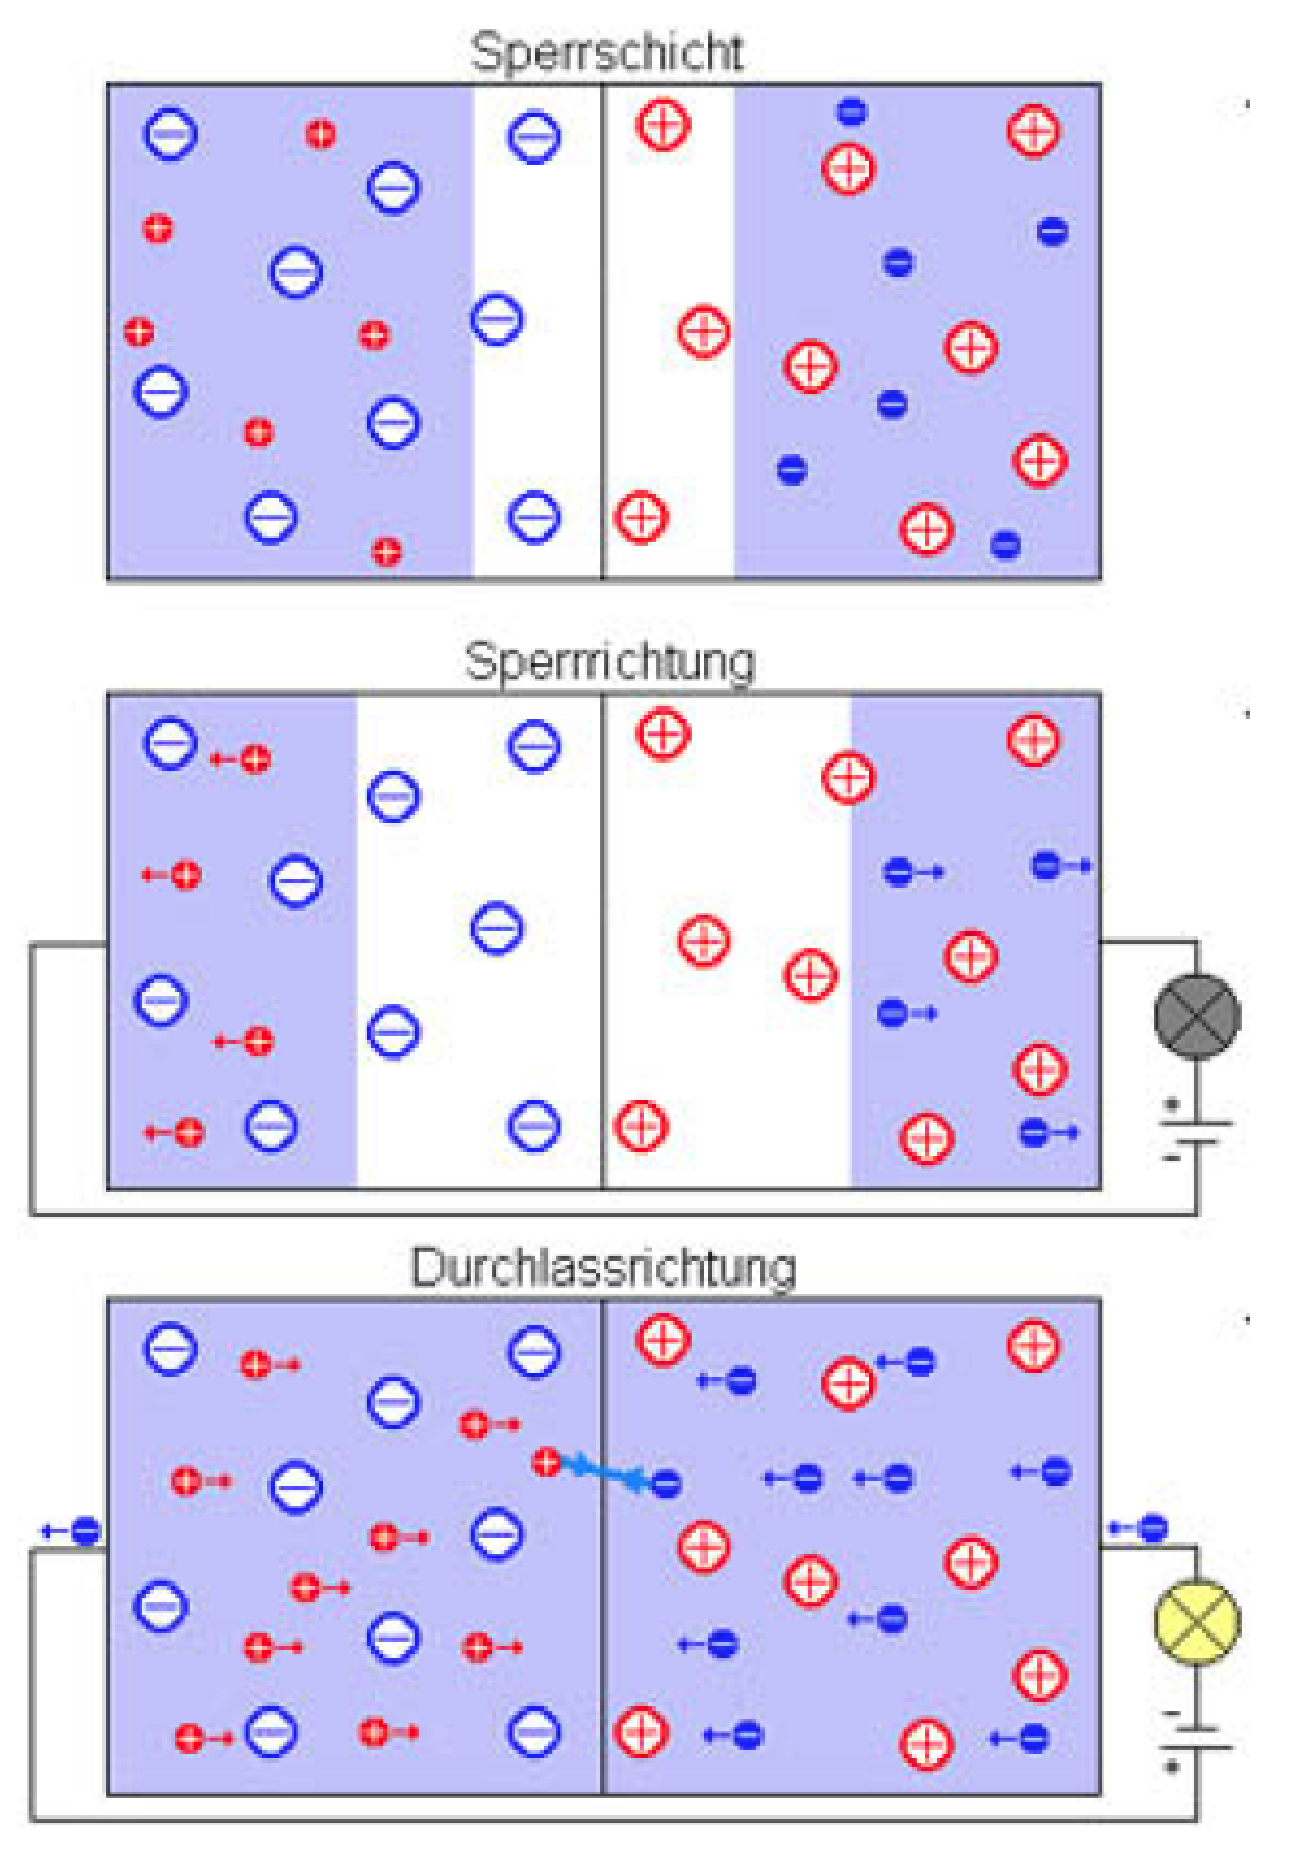
\includegraphics[scale=0.4]{sperrschicht.eps}
\caption{Oben: Sperrschicht mit Löchern (kleines Plus), freien Elektronen (kleines Minus) und Atomrümpfen (große Kreise). Mitte: Einbindung in einen Stromkreis in Sperrrichtung. Unten: Einbindung in einen Stromkreis in Durchlassrichtung.}
\label{fig:sperrschicht}
\end{figure}
\end{center}


\subsection{Eigenschaften verschiedener Dioden}
In diesem Experiment werden drei verschiedene Dioden verwendet: Si-Diode, Zener-Diode und LED.\\
Die Si-Diode (Silizium) funktioniert so wie oben beschrieben.\\
Die Zener-Diode hat eine genau spezifizierte Durchbruchspannung (Zenerspannung), die normalerweise wesentlich kleiner ist als die gewöhnlicher Dioden.\\
Bei Leuchtdioden (LEDs) wird Energie in Form von Photonen frei, also Licht emittiert. Das passiert, wenn Elektronen mit Löchern rekombinieren. Die ausgesandte Strahlung hat eine bestimmte Frequenz, die der Differenz zwischen den Energieniveaus entspricht, zwischen denen der Übergang stattfindet: $hf = E_1 - E_2$.\\
\\
Eine Diode hat eine Strom-Spannungskennlinie, die mit der Shockley-Gleichung beschrieben werden kann:
\begin{equation}
I_D=I_S\cdot\left(\exp^{\frac{U_A e \beta}{n}}-1\right)
\label{shockley}
\end{equation}
wo $\beta e=26\si{mV}$ bei Raumtemperatur ($T=300$K)

\subsection{Diode als Gleichrichter}
Wie oben bereits beschrieben kann eine Diode in Sperr- und Durchlassrichtung in einen Stromkreis geschalten werden. Aus diesem Grund kann man sie auch als Gleichrichter verwenden, um Wechselspannung in Gleichspannung zu verwandeln. Es kommen also am dazugeschaltenen Lastwiderstand  nur die positiven Halbwellen der Eingangsspannung an. Es handelt sich somit um eine pulsierende Gleichspannung.\\
Um die Spannung zu glätten kann ein Kondensator dazugeschalten werden. Während die Diode Strom durchlässt lädt der Kondensator sich auf (positive Halbwelle), während der negativen Halbwelle entlädt er sich über den Lastwiderstand. Daher entsteht am Lastwiderstand eine Last-Ausgangsspannung $U_a$, die von einer sogenannten Brummspannung $U_{BrSS}$ überlagert wird.\\
Die Brummspannung kann berechnet werden mittels: $U_{BrSS}=U_{a,max}-U_{a,min}$\\



\section{Aufbau und Durchführung}
Für fast alle Messungen wird das RC2000 Messsystem verwendet. Zur Messung des Spektrums der LEDs werden ein automatisches Spektrometer und das Programm SpectraSuite verwendet.

\subsection{Eigenschaften verschiedener Dioden}
Abbildung \ref{fig:diodenschaltung} zeigt den Messaufbau, um die Strom-Spannungs-Kennlinien verschiedener Dioden zu messen. Als Diode wird eine Si-, eine Zener-Diode bzw. eine LED verwendet. Als Vorwiderstand wird ein Ohm'scher Widerstand von 1k$\Omega$ verwendet.

\begin{center}
\begin{figure}[H]
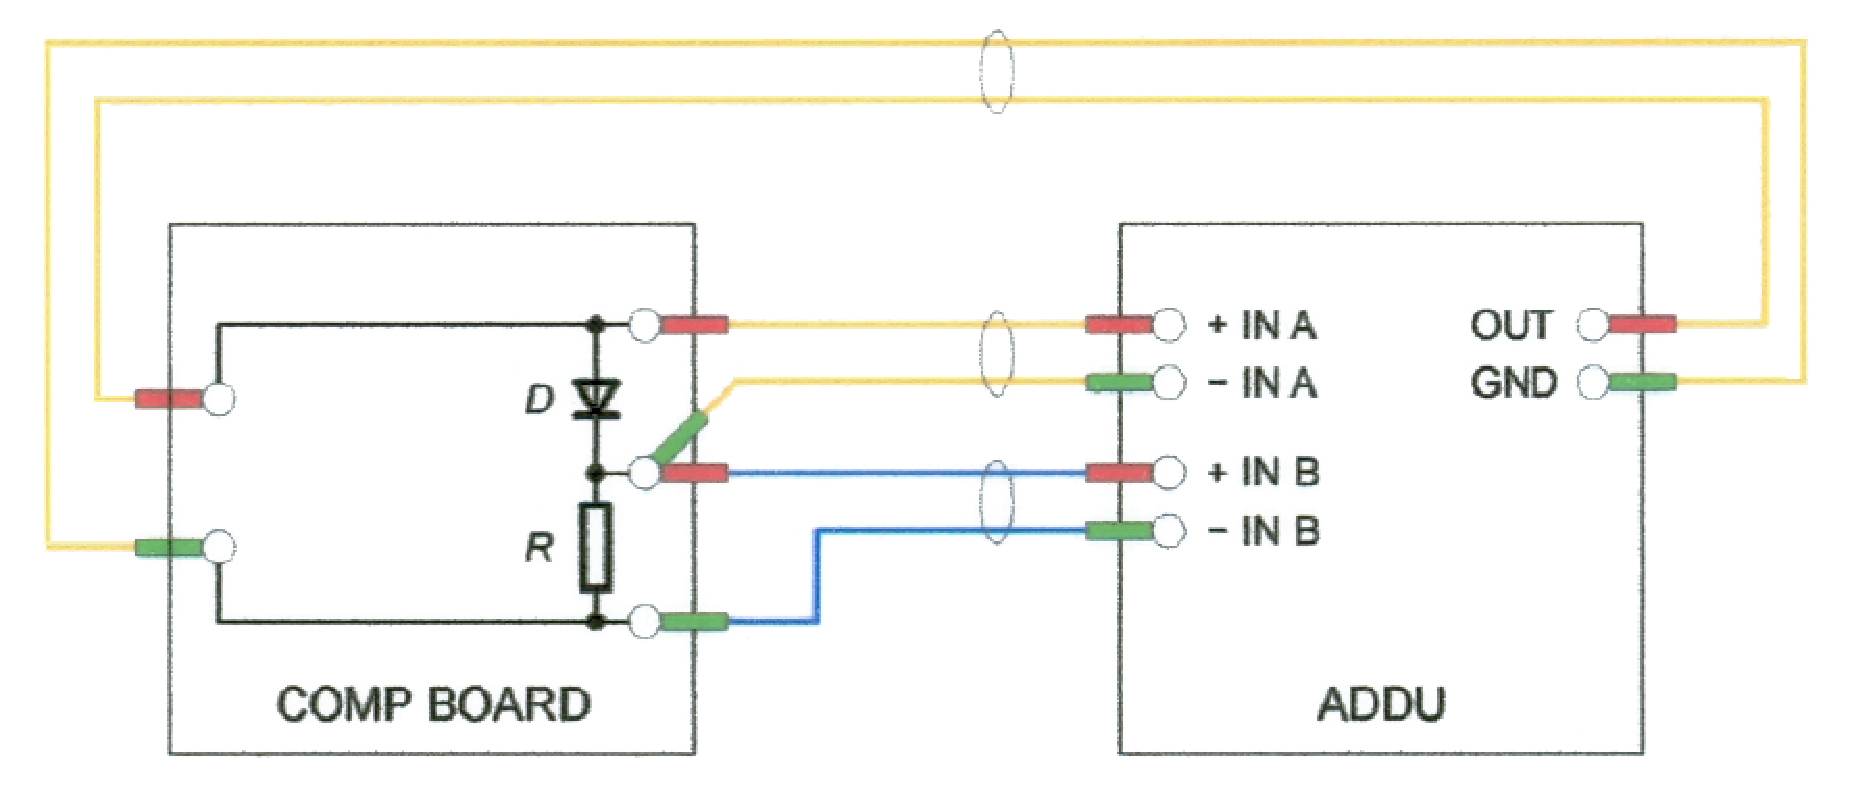
\includegraphics[scale=0.4]{schaltung.eps}
\caption{Aufbau zur automatischen Aufbau von Strom-Spannungs-Kennlinien}
\label{fig:diodenschaltung}
\end{figure}
\end{center}

Mit dem Messprogramm RC2000, Programmteil 'V-A-Characteristics', können die Strom-Spannungs-Kennlinien aufgezeichnet und ausgedruckt werden. Zur Messung der Wellenlänge der LEDs wird der Schrumpflschlauch des Spektrometers über die LED gestülpt und im Programm SpectraSuite eine Aufnahme des Signals gemacht. 

\subsection{Diode als Gleichrichter}

Abbildung \ref{fig:gleichrichter} zeigt die Schaltung, die für dieses Experiment verwendet wird.\\
Die Beschriftung 'rot'/'grün' bezieht sich nur auf den Aufbau mit vier LEDs: hier wurden für die positive Halbwelle zwei rote, für die negative Halbwelle zwei grüne LEDs verwendet, um eine schönere Kurve zu erhalten als mit verschiedenfarbigen LEDs möglich wäre. 

\begin{center}
\begin{figure}[H]
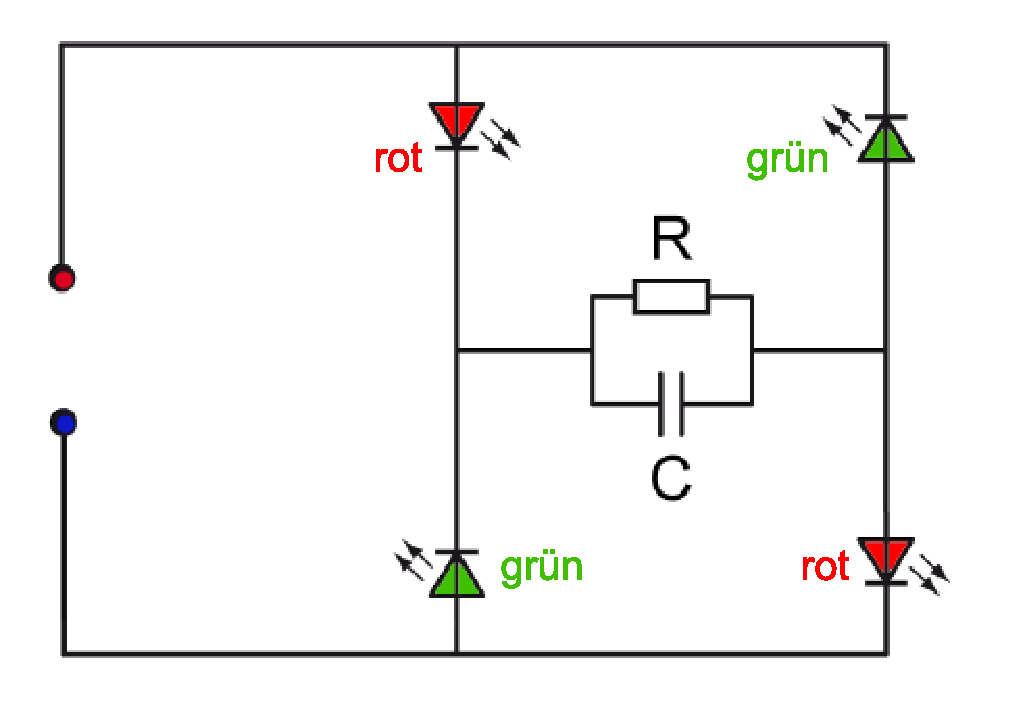
\includegraphics[scale=0.4]{gleichrichter.eps}
\caption{Schaltskizze eines Brückengleichrichters mit LEDs.}
\label{fig:gleichrichter}
\end{figure}
\end{center}

Mit dem Messprogramm RC2000, Programmteil 'Zweistrahl-Oszillograph', können die Last-Ausgangsspannung und Brummspannungen aufgezeichnet und anschließend ausgedruckt werden.

\section{Ergebnisse und Diskussion}
\subsection{Eigenschaften verschiedener Dioden}
%Strom-Spannungs-Kennlinie von R
\subsubsection{Unbekannter Widerstand}
Die Strom-Spannungs-Kennlinie eines unbekannten Widerstandes ist in Anhang 1 zu sehen. Eigentlich weiß man aus der Aufschrift des Widerstandes, dass er einen Wert von $R_x=2 k\Omega$ hat. Das soll aber auch mit dem Programm bestimmt werden können:\\
In der Strom-Spannungskennlinie ist, aufgrund des Ohm'schen Gesetzes, der Widerstand der reziproke Wert der Steigung der Geraden: $I=\frac{1}{R_x}\cdot U$. \\
Im Anhang ist der vom Programm berechnete Wert zu sehen: $R_x=2000\Omega$ bei $U_2-U_1=2.120\si{V}$ und $I_2-I_1=1.06\si{mA}$. Die Werte für $U_1$, $I_1$ und $U_2$, $I_2$ wurden jeweils mit der Cursor-Funktion des Programms ausgewählt; dabei wurde zur Verringerung der Unsicherheit der Abstand zwischen den beiden Punkten so groß wie möglich gewählt.\\
Wird als relative Unsicherheit jeweils 1\% des Messwertes verwendet, kann die absolute Unsicherheit des Widerstands berechnet werden. Da aber die relative Unsicherheit von $U_2$ genau $\Delta U_2=0.01\cdot U_2$ ist und selbiges in der Fehlerfortpflanzung wieder durch $U_2$ dividiert werden muss (und dies gilt auch für die anderen Werte) erhalten wir:
$\sqrt{0.01^2 + 0.01^2}=\sqrt{2}\cdot0.01=\Delta R_x$ (relativ).
Daraus erhalten wir, jetzt mit der absoluten Unsicherheit, das endgültige Ergebnis für den Widerstand: 

$$\boxed{R_x=(2000 \pm 28)\Omega}$$

Das Ergebnis für den unbekannten Widerstand ist wie erwartet passend; die Messung diente ja auch nur dem Zweck, sich mit dem System vertraut zu machen.

%Kennlinie einer Si-Diode; Fit mit Shockley-Gleichung in Durchlass-Richtung

\subsubsection{Si-Diode}
Die vom Programm aufgenommene Strom-Spannungs-Kennlinie einer Si-Diode ist in Anhang 2 zu sehen.\\
Im folgenden Plot ist ebenfalls die Strom-Spannungs-Kennlinie der Si-Diode sowie ein Fit mit der Shockley-Gleichung (\ref{shockley}) eingezeichnet. 
Die Werte von 
$$I_D=I_S\cdot\left(\exp^{\frac{U_A e \beta}{n}}-1\right)$$
sind dann $I_D$ als y-Achse, $U_A$ als x-Achse und 
$$I_S=(0.87 \pm 0.19)\mu A$$
$$n=3.51 \pm 0.01$$
Die Unsicherheit von $I_S$ beträgt fast 23\%. Man sieht Abbildung (\ref{fig:shockley}) auch an, dass der Fit nicht ganz zu den Datenpunkten passt. 

\begin{center}
\begin{figure}[H]
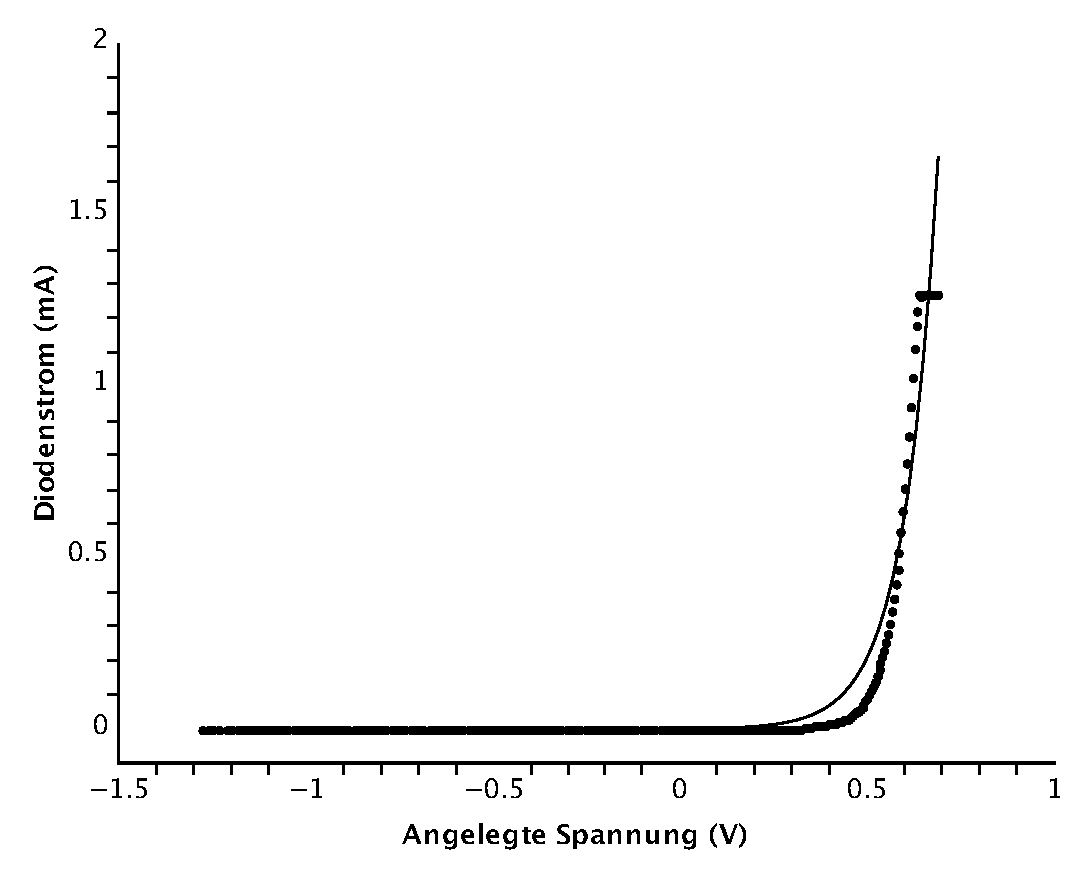
\includegraphics[scale=0.8]{shockley.eps}
\caption{Strom-Spannungs-Kennlinie einer Si-Diode und Fit mit der Shockley-Gleichung.}
\label{fig:shockley}
\end{figure}
\end{center}

%Kennlinien 4 verschiedener Zener-Dioden; Zenerspannung bestimmen (I=-1mA)

\subsubsection{Zener-Dioden}
In Anhang 3 sind die I-U-Kennlinien vier verschiedener Zener-Dioden zu sehen. Mit der Cursor-Funktion wurde der Wert von $I=-1\si{mA}$ angepeilt; da aber in keinem Fall ein Messwert an exakt diesem Punkt gemacht wurde, kann nur der nächstbeste Wert verwendet werden. Die zugehörigen Spannungen lauten dann wie folgt:

\begin{table}[H]
\centering
\begin{tabular}{|c||l|l|}
\hline
Diode & I (mA) & U (V)\\
\hline
4V3 & $-0.98 \pm 0.01$ & $-3.73 \pm 0.04$\\
3V6 & $-1.01 \pm 0.01$ & $-3.00 \pm 0.03$\\
2V4 & $-0.97 \pm 0.01$ & $-1.90 \pm 0.02$\\
3V0 & $-1.05 \pm 0.01$ & $-2.48 \pm 0.02$\\
\hline
\end{tabular}
\caption{Zener-Spannung U der Dioden bei $I\approx -1$mA}
\end{table}

%Kennlinien von 4 LEDs
%Optisches Spektrum der 4 LEDs mit einem automatischen Spektrometer; Kommentar zum Zusammenhang des Spektrums mit dem Kennlinienverlauf

\subsubsection{LEDs}
In Anhang 4 und 5 sind die I-U-Kennlinien sowie die Spektren von vier verschiedenen LEDs zu sehen. Die Farben der I-U-Kennlinien wurden passend zur Farbe der LEDs gewählt; bei den Spektren ist das nicht der Fall, allerdings erkennt man hier natürlich anhand der Wellenlänge, um welche LED es sich handelt. 

\begin{table}[H]
\centering
\begin{tabular}{|c|l|}
\hline
 & $\lambda$(nm)\\
\hline
Blau & $465 \pm 10$\\
Grün & $565 \pm 10$\\
Gelb & $588 \pm 10$\\
Rot & $643 \pm 10$\\
\hline
\end{tabular}
\caption{Wellenlängen zu den Dioden}
\end{table}

In Anhang 4 ist direkt ersichtlich, dass die Strom-Spannungs-Kennlinien der Reihe nach zu den Wellenlängen der LEDs gehören - Rot ($643\pm10$nm) benötigt die geringste Spannung, Blau ($465\pm10$nm) die höchste. Das ist darauf zurückzuführen, dass die Spannung erhöht werden muss, wenn eine höhere Energiedifferenz vorliegt, die umgekehrt proportional zur Wellenlänge ist. Daraus ergibt sich, wie in den Daten zu sehen, dass bei kleiner Wellenlänge höhere angelegte Spannungen benötigt werden.\\
\\
\\
Alle Strom-Spannungs-Kennlinien sehen aus wie erwartet.\\
Die Messung der LEDs war meiner Meinung nach besonders interessant, da der Zusammenhang zwischen Wellenlänge und Spannung gut zu sehen war. 

\subsection{Diode als Gleichrichter}
\subsubsection{Brückengleichrichter mit vier LEDs}
Anhang 6 zeigt die Eingangsspannung (A, gelbe Linie) und die Last-Ausgangsspannung (B, blaue Linie) in Abhängigkeit der Zeit.\\
Hier sieht man auch, dass die negative Halbwelle nach oben geklappt ist (blaue Linie).\\ Da es sich um verschiedenfarbige LEDs handelt, sind die Halbwellen unterschiedlich hoch (unterschiedlich hohe Spannung). Aus dem ersten Experiment kann man herleiten, dass die höhere Spannung zu den grünen LEDs, die niedrigere zu den roten LEDs gehört.\\
Der Strom-Fluss für beide Halbwellen ist in folgenden Diagrammen zu sehen:
\vspace{7cm}
\\Im Experiment konnte dieser Stromfluss auch gesehen werden, da abwechselnd die roten (Diagramm 1) und die grünen (Diagramm 2) LEDs geleuchtet haben. 

\subsubsection{Brückengleichrichter mit Si-Dioden}
Anhang 7 enthält die Eingangsspannung (A, graue Linie), die Last-Ausgangsspannung ohne Glättungskondensatoren (B, gelbe Linie), die Last-Ausgangsspannung mit einem 1$\mu$F Glättungskondensator (C, blaue Linie) und die Last-Ausgangsspannung mit einem 10$\mu$F Glättungskondensator (D, grüne Linie). \\
Die Brummspannung $U_{BrSS}$ kann aus den Werten im Anhang berechnet werden:

\begin{table}[H]
\centering
\begin{tabular}{|c|c|c|l|}
\hline
C ($\mu$F) & $U_{max}$ (V) & $U_{min}$ (V) & $U_{BrSS}$ (V)\\
\hline
- & $8.8$ & $0.0$ & $(8.8 \pm 0.08)$\\
1 & $8.8$ & $6.1$ & $(2.7 \pm 0.14)$\\
10 & $8.6$ & $8.3$ & $(0.3 \pm 0.16)$\\
\hline
\end{tabular}
\caption{Brummspannung bei einem Brückengleichrichter mit Si-Dioden}
\end{table}

\subsubsection{Variabler Lastwiderstand}
Leider Zettel mit Daten verloren.

						
\end{document}
